\chapter{Implementation}
During this chapter I will elaborate on the practical implementation of an application that will be used to prove the concept of the research.
The application is implemented in Flutter, a cross-platform framework developed by Google.
Due to the nature of the research and my hardware, the application is developed for Android and Linux devices only, and it will use a self-implemented server,
rather than a third party service such as Firebase.
\par
The server is implemented in Golang, a statically typed language developed by Google.
It will be used to store the data of the application, and to provide the necessary data to the application.
The server connects to a MSSQL database, which is used to store the data. 
This was also chosen due to nature of the research, as it represents a more realistic scenario, where the data is stored in a company's database.
Due to its ownership by Microsoft, a well-known brand, it is more likely to be used in a company's environment.
This is a good opportunity to test the application in a more realistic scenario, where the so-called 'frontend' and the 'backend' are not part of the same ecosystem.

\par
Let's now take a look at how the server and the application are implemented.

\section{Server}
The server is separated into the following main layers: Models, Database Operations, Controllers, and Middleware.
They are meant to provide core functionality to the server, and to separate the concerns of the application.
The middle layers are: Globals, Initializers, and Utils.
They are meant to provide support to the main layers, so that we can effectively separate the concerns. 
The purpose of having side layers is that we can easily declutter the main layers, and make the code more readable and maintainable.
Let's take for example the above utils function that helps us to display the error messages in a response body.
This will help us reduce boilerplate code, that is repeatable and makes the code harder to read.

\begin{figure}[htbp]
    \centering
    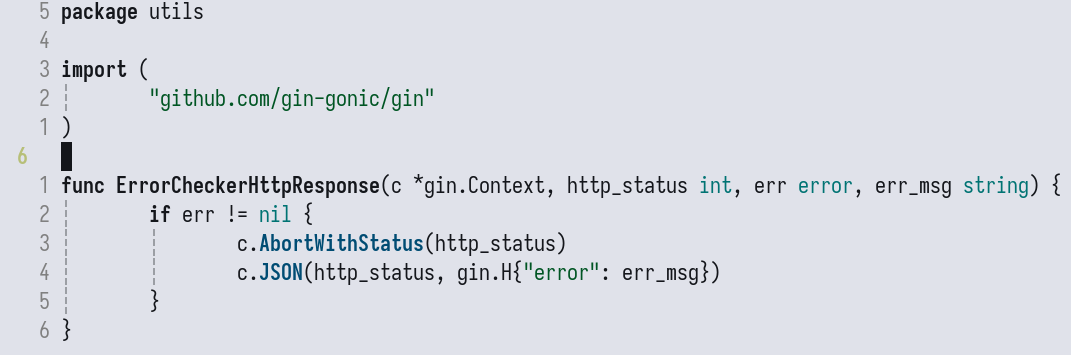
\includegraphics[scale=0.4]{pictures/server_utils.png}
    \caption{Utils layer}
    \label{utilsExample}
\end{figure}

\par
The Models layer contains the structs that represent the entities of the application. 
The structs are used to store the data of the application, and to provide a way to interact with the data.
They also provide a schema of the database, as they are used for mapping the results of the database queries.
Another use for them is to validate the data that is sent to the server, so that we can ensure that the data is correct.

\par
The Database Operations layer contains the functions that interact with the database.
They perform CRUD operations on the database, and to provide the necessary data to the application.
It is the layer that is responsible for the communication between the server and the database.
It's only functionality is the one mentioned above. Other logic, such as validation or error handling, is done elsewhere.
An advantage of writing this layer, instead of choosing and ORM (Object Relational Mapping) library, is that we have more control over the queries that are sent to the database.
This makes the server feel more responsive.

\begin{figure}[htbp]
    \centering
    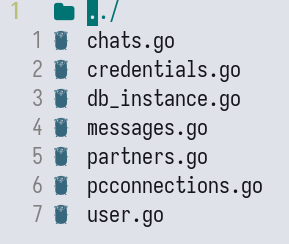
\includegraphics[scale=0.8]{pictures/dboperations.png}
    \caption{Database Operations layer}
    \label{dbOpsExample}
\end{figure}

\par
The Middleware layer goes between the Controllers and the endpoints calls.
It handles the logic that is common to all the endpoints, such as authentication, logging, and error handling.
This makes it easier to add new endpoints, as we don't have to write the same logic for each endpoint.
Also, the handlers for the endpoints can be easily replaced or removed, as they are not tied to the endpoints themselves.

\begin{figure}[htbp]
    \centering
    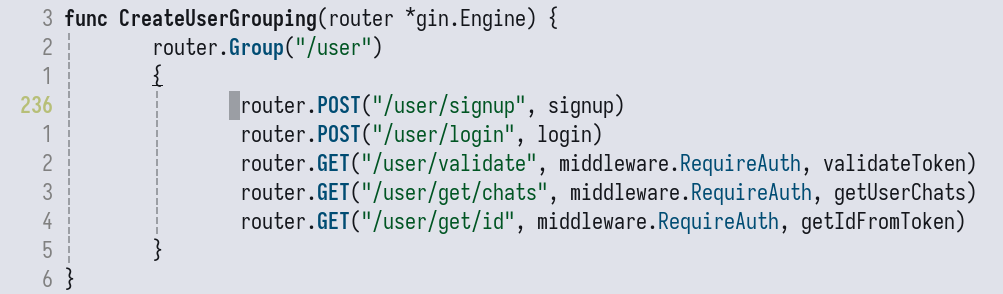
\includegraphics[scale=0.4]{pictures/middleware.png}
    \caption{Middleware layer}
    \label{middlewareExample}
\end{figure}

\par
The Controllers layer contains the functions that handle the requests from the client.
They are used to provide the necessary data to the client, and to handle the data that is sent to the server.
It is the main layer of the server, as they are the ones that interact with the client.
A key point of this layer is that it is not tied to the database, as it only interacts with the Database Operations layer.
I also chose to implement the controllers in a model-based way, as it makes the code more readable and maintainable.

\begin{figure}[htbp]
    \centering
    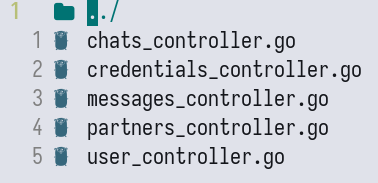
\includegraphics[scale=1.2]{pictures/controllers.png}
    \caption{Controllers layer}
    \label{controllersExample}
\end{figure}

\section{Main focus}
The main entity around which the application is built is the \textit{Partner} class, as seen below.

\begin{figure}[htbp]
    \centering
    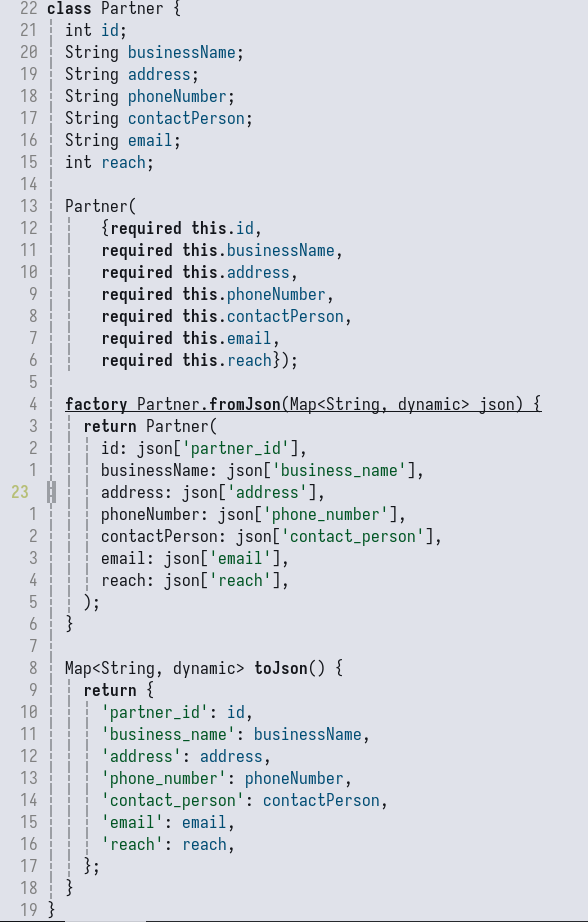
\includegraphics[scale=0.4]{pictures/partner_class.png}
    \caption{Main entity of the application}
    \label{partnersClass}
\end{figure}

This entity is a substitute for the User class, as the User is just a Partner connected with a Credential entity from the DB.
Partner is also connected to the entity Chat, which by itself is connected to Message.
This enforces a good separation of the functionality, and also allows for efficient queries and server responses.
Although this is the main entity, the way it is build, with the additional methods of \textit{fromJson} and \textit{toJson}, allows for easy extension of the application.
This will be present across all the other entities, to manage more easily the bodies of the sent requests.

\par
Now, we'll take a look at how a few components are built, and how their state is managed.
This will contain some good and bad examples, and see how they impact the development of the application, and also the developer experience.

\section{Example Components}
\subsection{Good example}
The first component we'll take a look at is a \textit{Partner list} component. 
To be more specific, the below picture is part of the component that renders the top five partners by reach, a field which represents the average number of clientele.

\begin{figure}[htbp]
    \centering
    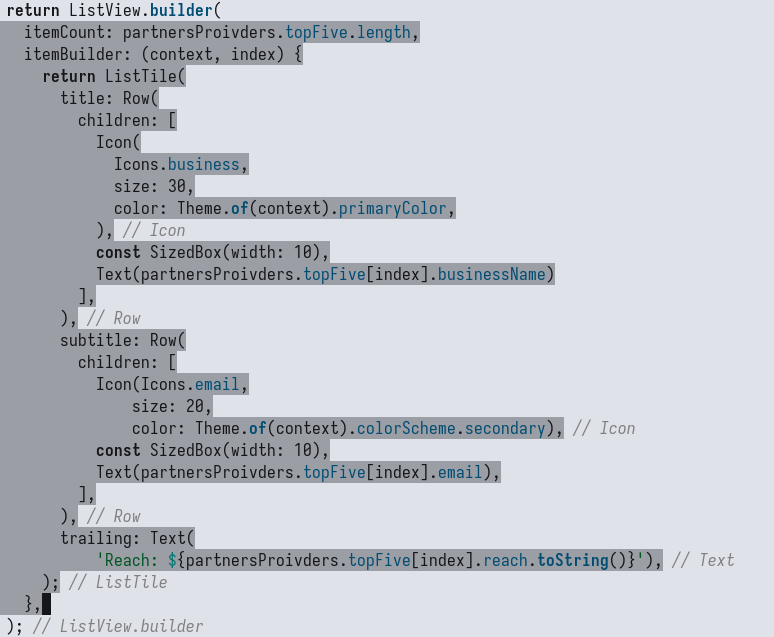
\includegraphics[scale=0.4]{pictures/partners_mapped_good_example.png}
    \caption{List component}
    \label{partnerListComponent}
\end{figure}

Here we can note the good use of states, as the component is stateless, and the state is managed by the provider component.
This is a good practice, as it allows for a more efficient rendering of the component, and also for a more readable code.
Each child sits under a \textit{Consumer} widget, which listens for changes in the provider, and rebuilds the child when the state changes.
By doing so, the component is more efficient, as only the child that needs to be rebuilt is rebuilt, and not the whole component.
Also, it removes for the need of passing the state as a parameter to the child.
Due to the simple nature of the entity is overwatches, it eliminates the need for a websocket.
This is a good example of how to build a component, and how to manage the state of the component, for simple operations on simple entities.

\newpage
\subsection{Bad example}
The second component we'll take a look at is a \textit{Login} component.
This component is used to log in the user, and to provide the necessary data to the application.
In the picture below, we can see that the component is stateful, through the use of controllers.
This is a bad practice, as it makes the component easy to read, but prone to mistakes, due to repetitve coding.

\begin{figure}[htbp]
    \centering
    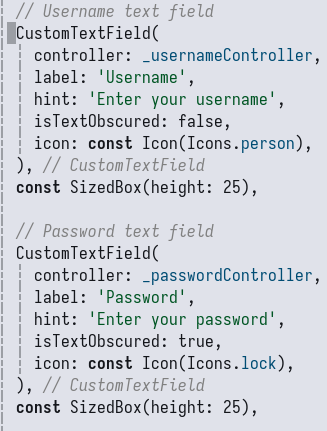
\includegraphics[scale=0.4]{pictures/looks_bad_but_is_good_because.png}
    \caption{Login component}
    \label{loginComponent}
\end{figure}


This is as much avoided as possible, through the makings of custom widgets, that eliminate boilerplate as much as possible.
It is easily observable in the picture below, where \textit{CustomTextField} is used to create a text field, with a custom design, and a custom controller.
Everything under the \textit{Widget build} method would be repeated for each text field, and would make the code harder to read and maintain.
\begin{figure}[htbp]
    \centering
    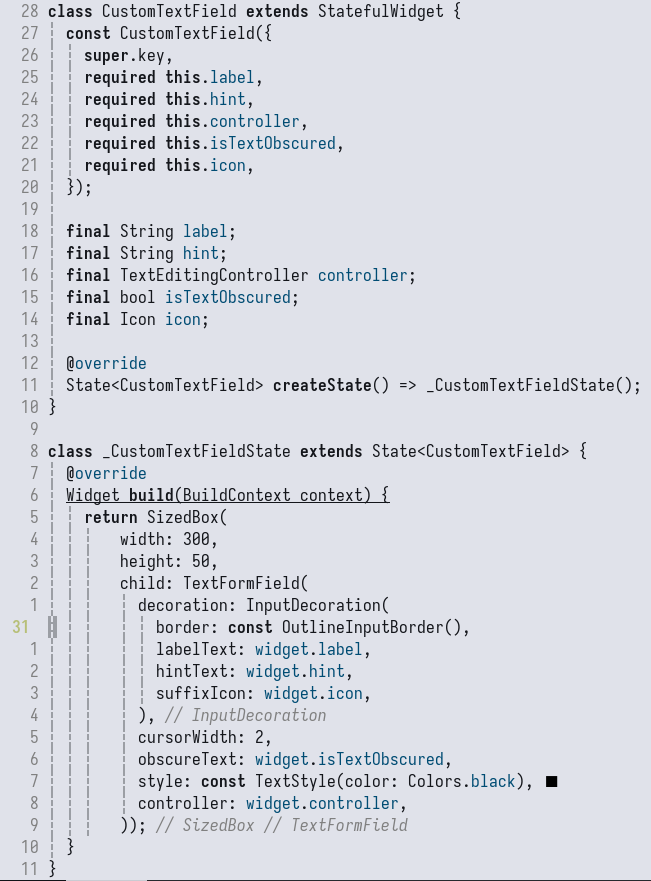
\includegraphics[scale=0.2]{pictures/it_avoid_boilerplate.png}
    \caption{Custom text field}
    \label{customTextField}
\end{figure}



\newpage
\subsection{Neutral example}
The last component we'll take a look at is a \textit{User Details} component.
This component is used to display the details of a user, such as the name, email, and phone number.
It also allows the user to edit the details, and to save the changes.
In the picture below, we can see that the component is stateless, and the state is managed by the \textit{Partners Provider}.

\begin{figure}[htbp]
    \centering
    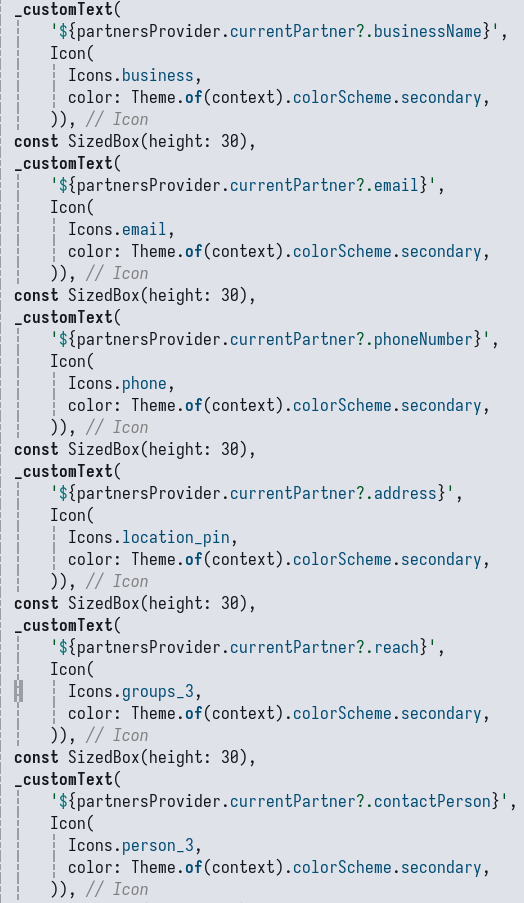
\includegraphics[scale=0.4]{pictures/partners_not_mapped_bad_example.png}
    \caption{User Details component}
    \label{userDetailsComponent}
\end{figure}

This is a bad practice, as it makes the component harder to read, and harder to maintain.
Also, it makes the component less efficient, as there is no need for the whole component to be rebuilt when the provider notifies for changes.
This example, although it is a simple one, shows how not to build a component, and how not to manage the state of the component.
This represents a tricky example, because it looks like a bad mapping, because it is done manually.
In reality, it provides a way to improve the design of the application, by giving custom icons to the inner components.
We can notice this in the picture below.

\begin{figure}[htbp]
    \centering
    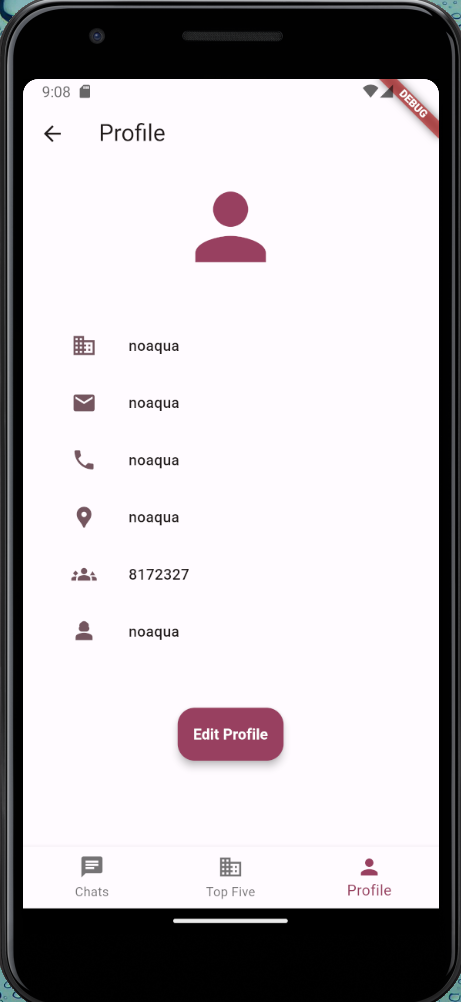
\includegraphics[scale=0.4]{pictures/because_it_looks_bad_we_have_ui.png}
    \caption{User Details UI}
    \label{userDetailsUI}
\end{figure}

\label{implementation}

